%=============================================================================
% Mechanism Is Not Meaning: A Verification Methodology for Cognitive-Architecture
% Prototypes.   IEEE CONFERENCE VERSION (IEEEtran, double-column, 4-6 pp).
%
% Target venues: IDAP / UBMK symposia (IEEE conference format, strict 4-6 page
% double-column limit).
%
% This is the CONDENSED conference rendering. The full preprint is the source of
% truth for every claim (../paper.tex); this version preserves the exact claims
% and calibration and only condenses. SKELETON ONLY for now: section headings
% plus a one-line content comment each, no body prose.
%
% PERMANENT CONSTRAINTS (identical to the preprint, from the locked claim
% inventory):
%  - Self-contained; no file paths, commit hashes, or repository pointers.
%  - No em-dashes (never three consecutive hyphens); en-dash (two hyphens) only
%    for numeric ranges in rendered text.
%  - Calibrated certainty per assurance tier: PROVEN / MECHANISM-VERIFIED /
%    METHODOLOGY / NOT-YET. Never claim mind, consciousness, sentience, AGI, or a
%    validated cognitive model (CC-1, CC-2). A NOT-YET is "could not be
%    established on this substrate," never "the phenomenon is absent" (CC-3).
%  - System name is "Psyche" in both the paper and the codebase.
%  - Numbers only from real sources; canonical suite is 20 suites / 1,372
%    assertions / 0 failures; substrate is 80 assertions (45 + 35).
%=============================================================================
\documentclass[conference]{IEEEtran}

% Encoding and fonts (Turkish glyphs in the author name render under
% pdfLaTeX via utf8 input + T1 output encoding; no Unicode engine needed).
\usepackage[utf8]{inputenc}
\usepackage[T1]{fontenc}
\usepackage{lmodern}

% IEEE-standard packages.
\usepackage{cite}                       % numbered [1],[2] citation handling
\usepackage{amsmath,amssymb,amsfonts}
\usepackage{graphicx}
\usepackage{booktabs}                   % clean rules for the condensed errors table

% Diagrams: the SAME shared palette and styles as the preprint so the ported
% figures match. Node sizes may be reduced when a figure is placed in a single
% IEEE column, or a wide figure moved to a two-column figure* float; those
% decisions belong to the body-writing phase.
\usepackage{tikz}
\usetikzlibrary{arrows.meta, positioning, calc}
\definecolor{pblue}{HTML}{39516B}
\definecolor{pred}{HTML}{8F3B3B}
\definecolor{pgrey}{HTML}{5A5A5A}
\tikzset{
  pnode/.style     = {draw=pgrey, line width=0.7pt, rounded corners=2pt, fill=white,
                      align=center, inner sep=4pt, font=\small, minimum height=8mm},
  pstage/.style    = {pnode, minimum width=16mm},
  prole/.style     = {pnode, minimum width=24mm, text width=24mm},
  ptier/.style     = {pnode, minimum width=70mm, text width=70mm, minimum height=10mm},
  paccent/.style   = {draw=pblue, line width=1.0pt},
  popen/.style     = {draw=pred, line width=0.9pt, dash pattern=on 3pt off 2pt},
  pdim/.style      = {draw=pgrey!55, dash pattern=on 2pt off 2pt, text=pgrey!85},
  pflow/.style     = {-{Stealth[length=2mm]}, draw=pgrey, line width=0.7pt},
  pfeedback/.style = {pflow, dashed},
  pedgelbl/.style  = {font=\footnotesize, text=pgrey, fill=white, inner sep=1.5pt},
  pnote/.style     = {font=\footnotesize, text=pgrey, align=center},
}

% Hyperlinks (load last; hidden so the IEEE print layout is unchanged).
\usepackage[hidelinks]{hyperref}

%=============================================================================
\begin{document}

\title{Mechanism Is Not Meaning: A Verification Methodology for
       Cognitive-Architecture Prototypes}

\author{\IEEEauthorblockN{Çağan Çalışkan}
  \IEEEauthorblockA{ORCID:~\href{https://orcid.org/0009-0000-2993-1421}{0009-0000-2993-1421}}}

\maketitle

\begin{abstract}
Building a cognitive-architecture prototype invites a recurring confusion between two claims
that resemble each other: that a mechanism is correct, and that it carries meaning. The
pressure to overclaim is strongest when a system can be graded on inputs chosen to make it
succeed. This paper presents a verification methodology that holds the two apart, demonstrated
on Psyche, a dependency-free substrate assembled into a closed cognitive cycle. The methodology
combines four practices: a separation of duties between building and certifying, loop-closure
driven by system-generated input, adversarial and property-based testing, and pre-registration
with anti-circularity gates. Under it, the substrate's properties are proven and the cycle is
verified as a mechanism, with no cognitive claim. The methodology is then exercised on three
attempts at an externally graded cognitive result: semantic priming, the fan effect, and an
interoceptive modulation. Each was halted before any graded number, for a structurally distinct
reason. The recurring obstacle, the relationship between the mechanism and an external yardstick
rather than the mechanism itself, is the finding. The meaning bar was not cleared; the results
concern method and mechanism, not cognition.
\end{abstract}

\begin{IEEEkeywords}
verification methodology, cognitive architecture, property-based testing,
pre-registration, reproducibility, spreading activation
\end{IEEEkeywords}

%=============================================================================
\section{Introduction}\label{sec:intro}
A system built toward cognitive claims is under steady pressure to be described as
more than it is. Each working mechanism invites a larger reading, and the least
demanding way to support that reading is to grade the system on inputs chosen to make
it succeed. The result is a recurring confusion between two statements that resemble
each other and are not the same: that a mechanism is correct, and that it carries
meaning. Holding them apart is a methodological problem before it is a scientific one,
and it is the problem this paper addresses. The contribution is a verification
methodology for building cognitive-architecture prototypes without the overclaiming,
carried from the substrate upward through one such prototype.

The prototype is Psyche.
It is a dependency-free substrate, a graph store and a spreading-activation
engine, assembled into a closed cognitive cycle. It was built under a longer-term
interest in biologically-motivated, non-LLM cognitive architectures, but that motivation
is not what this paper evaluates. Two grades of evidence are kept apart throughout. The
substrate's properties are proven: deterministic across separate processes, internally
consistent through every change, and free of any read that alters stored state. The
cycle above it is verified as a mechanism and nothing more; it is not claimed to
perceive, to attend, or to mean. Naming it a cognitive cycle borrows a control structure
from an established tradition and asserts nothing about cognition.

The methodology is four practices. A separation of duties keeps the role that writes a
mechanism from the role that certifies it. Loop-closure drives each stage with the input
the previous stage produced, not input placed by hand. Adversarial and property-based
testing asserts invariants designed to break a claim rather than to confirm it.
Pre-registration with anti-circularity gates fixes a prediction and its direction before
any graded number is computed. None of the four is novel alone; their combination, turned
on a developer's claims about a system they are building, is the contribution.

The discipline is tested where the temptation to overclaim is strongest: at the step from
a working mechanism to an externally graded cognitive result. Three times the project
reached for such a result against data it did not author, attempting semantic priming, the
fan effect, and an interoceptive modulation. Three times the anti-circularity gates
refused the attempt before any graded number existed, and each time for a structurally
distinct reason: one claim could not be separated from the construction of the substrate,
one named a generating mechanism the engine does not contain, and one rested on a signal
that does not vary on the work the system does. That three independent attempts halted at
the same place, the join between the mechanism and an external yardstick rather than the
mechanism itself, is the finding. The meaning bar was not cleared, and this paper does not
present it as cleared; it reports a result about method and about mechanism.
Section~\ref{sec:substrate} describes the substrate and the closed cycle,
Section~\ref{sec:methodology} the methodology, Sections~\ref{sec:attempts}
and~\ref{sec:metafinding} the three attempts and what they share, and
Sections~\ref{sec:limrelated} and~\ref{sec:conclusion} the limitations, related work, and
conclusion.

%=============================================================================
\section{The Substrate and Closed Cycle}\label{sec:substrate}
Psyche is built in two layers carrying two grades of evidence. The lower layer, the
substrate, is a graph store with a spreading-activation engine; its properties are
proven, in a precise sense: identical output across separate processes under randomized
hashing, mutual consistency of the graph indices after every mutation, and reads that
never alter stored state. The upper layer assembles the substrate into one loop,
perceiving, activating, clustering, selecting, pruning, and writing, whose stages are
verified as mechanisms but make no claim to reproduce a cognitive phenomenon. The loop is
called a cognitive cycle because its shape is taken from the global-workspace tradition
\cite{baars1988cognitive, franklin2014lida}, as a structural template; the term names a
control structure and asserts nothing about cognition.

The store is a directed graph whose nodes are concepts and whose roads are weighted,
directed connections carrying a strength, a usage record, and a decay with elapsed time.
The load-bearing decision is that reading and writing are separated at the level of decay.
An earlier arrangement applied decay at the moment of access and wrote the decayed value
back, with two consequences a casual reading misses: every read mutated the store, and,
because the same step re-evaluated closure, a run of reads over time could let a closed
road drift back open although nothing crossed it. Psyche instead splits decay into a pure
view and a persisting write. A read returns a decayed copy computed from elapsed time but
stored nowhere, so reading changes nothing, while only active operations persist a decayed
value, and closure is re-evaluated only on an active crossing, never by elapsed time or by
a read. The substrate is proven to hold these properties: reads are pure, closure does not
drift, the indices stay consistent through every insertion and deletion including on
adversarially constructed graphs, and a deletion leaves no dangling entry.

Activation is the substrate's one dynamic operation: given seed nodes, the engine
propagates a diminishing quantity along the roads and reports how much each reached node
accumulates. The mechanism is the spreading activation of ACT-R \cite{anderson1998atomic},
borrowed without that architecture's empirical commitments, and two choices make it well
defined. The first is bounded single-expansion: each node expands once, at the first hop it
is reached, carrying the full sum of all equal-length paths, so activation that converges is
summed once and exactly rather than re-counted downstream of the convergence. The second
secures determinism: the engine expands hop by hop and freezes each layer before it acts, so
no node observes another's expansion within a layer and the outcome cannot depend on the
order in which nodes or roads are visited. The engine is in consequence deterministic across
separate processes under randomized process hash seeds (5--8 per suite, in fresh
interpreters) and, like the store, computes as a pure read. Together the store and the engine
form the proven substrate; their two suites contribute 45 and 35 assertions, 80 in all,
within a verification suite that stands at 20 suites and 1{,}372 assertions with no failures.

Above the substrate, Psyche arranges these operations into a single loop
(Figure~\ref{fig:cycle}). A cycle begins by perceiving: the input text is matched against
the substrate, and the named nodes become the cycle's sources. This is what makes the loop
a genuine test rather than a staged one, because the sources are produced by the system from
its own contents rather than placed by hand. Because perception names sources that lie close
together, the first stage groups them before any field is built, merging by single linkage
\cite{sibson1973slink} on road strength alone, so the grouping is topological and does not
encode the answer the later stages compute. The engine then builds its field over the
grouped sources, the co-activated region is partitioned into candidate coalitions, and
exactly one is selected by a competition normalized for coalition size, so a coalition does
not prevail merely by being large. Selection then prunes any region the winner reaches across
a single bridge into territory the input never named, keeping a reached element only where it
attaches at least as strongly to the named region as to the unnamed one. The rule is
parameter-free and its one divergence is on the safe side: an unnamed region bridged at least
as strongly as it coheres internally presents no valley to cut and is retained, so the rule
may over-include an unnamed region but never prunes a member the input named.

\begin{figure}[t]
  \centering
  \resizebox{\columnwidth}{!}{%
  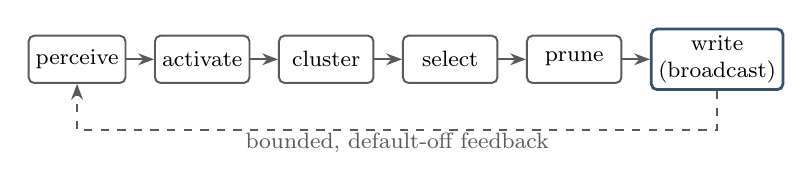
\begin{tikzpicture}[node distance=3.5mm,
      pstage/.append style={minimum width=12mm, minimum height=6mm, inner sep=2.5pt,
                            font=\footnotesize}]
    \node[pstage] (s1) {perceive};
    \node[pstage, right=of s1] (s2) {activate};
    \node[pstage, right=of s2] (s3) {cluster};
    \node[pstage, right=of s3] (s4) {select};
    \node[pstage, right=of s4] (s5) {prune};
    \node[pstage, right=of s5, paccent] (s6) {write\\(broadcast)};
    \draw[pflow] (s1) -- (s2);
    \draw[pflow] (s2) -- (s3);
    \draw[pflow] (s3) -- (s4);
    \draw[pflow] (s4) -- (s5);
    \draw[pflow] (s5) -- (s6);
    \draw[pfeedback] (s6.south) -- ++(0,-5mm) -| (s1.south);
    \node[pnote] at ($(s1.south)!0.5!(s6.south)+(0,-7mm)$) {bounded, default-off feedback};
  \end{tikzpicture}%
  }
  \caption{The closed cycle of Psyche at the level of mechanism: perception and activation,
    clustering of the perceived sources, selection of one coalition, bridge pruning, and a
    single bounded write, the broadcast, that biases the next cycle. The feedback is bounded
    and off by default. The figure depicts graph operations and one bounded write, with the
    verbs select, prune, and write, not decide, attend, or experience, and makes no cognitive
    claim.}
  \label{fig:cycle}
\end{figure}

Up to here the cycle has only read the substrate. Its one write is the broadcast: the
winning coalition is reinforced on its internal roads, biasing the next cycle toward the
same region. The reinforcement reuses the store's strengthening rule, which adds to a road's
strength a fixed fraction of the distance remaining to its ceiling,
\begin{equation}
  s \;\leftarrow\; s + \gamma\,(1 - s), \qquad 0 < \gamma \le 1,
\end{equation}
so each application closes part of the gap to $s = 1$ without ever reaching it. Boundedness
is therefore structural rather than imposed: the broadcast carries no cap, no ceiling test,
and no tunable magnitude of its own. With the broadcast off the loop is a pure read whose
output is byte-for-byte identical to the pre-broadcast pipeline; enabling it adds exactly one
bounded write per cycle. This is the precise content of the claim that the cycle closes: a
pipeline that runs to completion on its own output, deterministic and pure in its read
portion and bounded in its single write. Each stage, the clustering, the competition and
pruning, and the bounded broadcast, has been independently and adversarially re-verified for
determinism across randomized process hash seeds, integrity, and read-purity, and for none of
them is any cognitive claim entered.

%=============================================================================
\section{The Verification Methodology}\label{sec:methodology}
The substrate and the cycle are the case study; the contribution is the discipline that
determined what could be claimed about them, and at what grade of evidence. That discipline
counters one hazard: a project building toward cognitive claims is pressed to read more into
a working mechanism than it has earned, and the easiest way to do so is to grade the system
on inputs chosen to make it succeed. The methodology is four practices that force every claim
to earn its tier and hold two statements apart, that a mechanism is correct and that it
carries meaning, the first settled against hard properties and the second against external
data.

Two qualifications belong at the front. First, the four roles described below are AI
subagents operating under enforced lane rules within a single project directed by one person.
They are a separation of roles and contexts, not independent human teams and not external
auditors. Second, the discipline is reported as what it did, not as a guarantee: it caught
the errors recounted below and refused three premature claims, but it is demonstrated on one
system and establishes neither freedom from bugs nor that it would transfer.

The work is divided among four roles. An architect specifies each component together with the
external criterion by which it will be judged. A builder implements each specification
test-first. A separate tester then re-verifies the result, writing its own hostile and
loop-closed suites and never editing production code. A validator enters only when a
cognitive claim is at stake, grading it against external data under a prediction fixed in
advance. The reason for the division is that the role which writes a mechanism should not be
the role that certifies it: when author and certifier coincide, verification decays into
self-attestation, the tests coming to encode the author's own model of the code and passing
for the same reason the code was written. Holding the tester apart makes agreement between
builder and tester informative, because the tester was trying to falsify. The tester's checks
are largely property-based, asserting invariants that must hold across inputs of a kind, such
as determinism across processes, purity of reads, and integrity of the graph, in the
tradition of property-based testing \cite{claessen2000quickcheck, maciver2019hypothesis}.

The second practice governs the inputs a test may use. A test that hands a stage the input on
which it is expected to work can pass while the stage is structurally wrong, because it never
confronts the stage with anything it was not built to handle. Loop-closure requires instead
that each stage be driven by the input the previous stage actually produced. This removes the
author's choice of input, which is where self-deception enters: as long as the sources
feeding a stage are placed by hand, ``it works'' means only ``it works on my guess of its
input.'' Closing the loop forces each stage to consume the previous stage's real output, and
it was this substitution that exposed the errors below, several of which were invisible on
friendly inputs.

Applied together, adversarial re-verification and loop-closure caught a series of structural
errors, defects in the shape of the algorithm rather than the spelling of the code. Six are
on record; three are recounted here, and the claim is only that they were caught on this
system, not that the discipline finds every error. The first concerns the boundary between
reading and writing: computing decay at the moment of access and writing it back made every
read a mutation and, because the same step re-evaluated closure, let a closed road drift open
over a run of reads. A happy-path test passes this by, since reading the right value is what
it checks; the defect was caught by an assertion that a battery of reads leaves stored state
identical, and repaired by the pure-view and persisting-write split described above. The
second lay not in a mechanism but in how one was judged: an early community-recovery test
\cite{blondel2008fast, traag2019louvain} reported success only because a source had been
placed by hand at the centre of each community, so the answer was written into the input.
Closing the loop caught it; when sources were instead derived by perception from real input,
the same pipeline produced an incoherent result, and the original failure was preserved as a
standing assertion set to turn green only once the upstream grouping was genuinely fixed,
which it since has. The third was carried from a neighbouring problem: where activation
reaches a node along several paths the contributions must add, but a shortest-path intuition
re-expands the node and counts everything downstream of the convergence more than once, fixed
by bounded single-expansion with a locking check that the post-convergence value is the exact
sum. The remaining three were an order-dependence and an identity leak that made results swing
across process hash seeds, both removed by hop-layered expansion with frozen per-layer values
and a stable tie-break, and a binding degeneracy in which connected components on a graph
connected by construction yield a single group, resolved by reframing to a multi-source field.

The fourth practice governs claims about meaning, taken from the use of pre-registration in
empirical science \cite{nosek2018preregistration}. Before any graded number is computed, the
prediction and the direction it must take are fixed, and the artifacts of an experiment, its
stimulus lists and selection criteria, are content-hashed before any graded outcome exists;
stimulus selection is run blind, consuming only the structure of the data and never the
quantity against which it will be judged. If the prediction may be adjusted after the data are
seen, almost any outcome can be dressed as a confirmation, and the test loses its power to
discriminate. In this project the gates are not a formality: on each of three occasions a
cognitive claim was put to them, they returned a refusal before any graded number was
computed, because the design could not be populated or graded without circularity.

Taken together, the four practices form one stance toward the system's own claims. None of
this proves that Psyche is correct, that the next error would be caught, or that the
discipline transfers beyond this system. What it supports is the narrower claim this paper
makes: on this system, the discipline caught the structural errors recorded here and refused
three premature claims, and it did so by construction rather than by chance.

%=============================================================================
\section{Three Meaning-Bar Attempts}\label{sec:attempts}
Three times the project reached for an externally graded cognitive result, and three times
the gate declined to grade it. What makes this evidence rather than anecdote is that the
three refusals were not one obstacle met three times, but three structurally distinct
obstacles: a claim that could not be separated from the construction of the substrate, a
claim whose generating mechanism the engine does not contain, and a claim whose external
signal does not vary on a realistic workload. A discipline that halts for three different
reasons responds to the structure of each problem, not to a single recurring artifact.

Two points of calibration hold across all three. First, each finding concerns what could be
established on this substrate with this instrument, not the phenomenon in the world: none of
the three says, or licenses, that priming, the fan effect, or interoception is absent in
human cognition. Second, in none of the three was a graded result computed. No effect size,
no slope, and no direction of effect was produced; the gate fired at selection or at a
feasibility check, before the loop was run for score.

The first attempt was semantic priming, with relatedness drawn from a published corpus of
human word-association norms \cite{dedeyne2019swow} rather than from the system. The
difficulty is that the corpus encodes association strength as the weight of the edge between
two concepts, and Psyche's substrate is built from exactly those weighted edges, so a naive
result could appear to prime simply by reading back the edge weights it was constructed from.
The pre-registered design therefore required a weight-blind leverage stratum, prime pairs in
which the strong and weak associates carry equal edge weight and are matched for target
popularity, so that any measured difference would have to come from the loop. The gate was
whether that stratum could be populated. A blind selector, consuming only graph structure and
the published strengths and computing no activation, found 7 such pairs against a
pre-registered floor of 30, and the fallback statistic would have had to exceed its own
ceiling of 1 to register an effect. The calibrated finding is narrow: on this corpus, with
both the edge-weight and target-popularity paths controlled, priming-through-the-loop cannot
be separated from the substrate's own weight map. That is a statement about separability on
this corpus, not a claim that priming is absent.

The second attempt was Anderson's fan effect, the finding that the more associations a concept
acquires, the more slowly any one is retrieved \cite{anderson1974retrieval,
andersonreder1999fan}. It was chosen because it escapes the circularity of priming, riding on
the number of a concept's associations rather than the weight of any one. The reason it could
not be graded lies deeper, in what produces the effect. In the account it comes from
\cite{anderson1998atomic}, retrieval shares a fixed budget: a source emits a conserved quantity
of activation divided among its associations, so each receives less as their number grows.
Psyche's engine conserves no such budget; each outgoing road receives the source's full
activation, with no division by the number of roads. The consequence was measured: as the
number of associations is swept upward, the activation delivered to a target does not fall but
stays flat to the last digit, 0.2433743975, across the fan sizes tested
(Figure~\ref{fig:fanflat}). This is a different wall from the first. Priming was circular, and
the gate existed to keep a mechanical read-back from being mistaken for a loop effect; here
there is no signal to grade in any direction, because the mechanism that would generate one is
not in the engine. The two failures are in a sense opposites: the first had a confound to rule
out, the second has nothing to measure. An engine change that divides activation among a
source's roads would create a fan effect, but it is held as a separate architectural decision,
not a repair undertaken to produce the result, and adopting it to obtain the effect would not
earn it. The calibrated finding is again narrow: the fan effect is not produced by the engine
as Psyche builds it, which says nothing about the fan effect in human memory.

\begin{figure}[t]
  \centering
  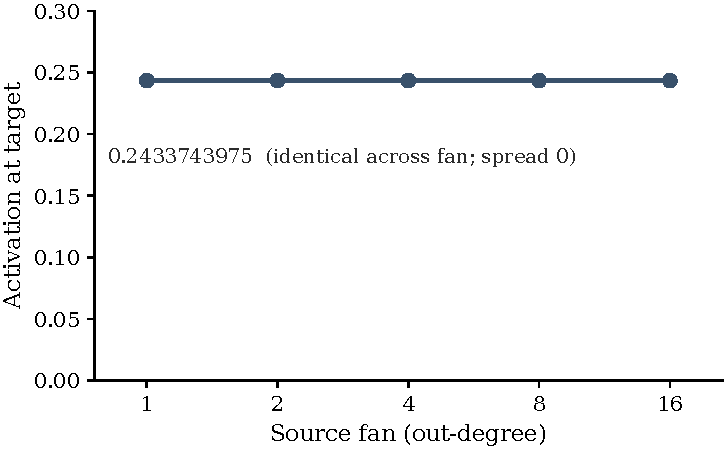
\includegraphics[width=\columnwidth]{figs/fan_flat.pdf}
  \caption{The fan-effect attempt: the activation delivered to a target is flat across fan
    size. As the number of a concept's associations grows over the sizes tested, the target's
    activation does not change to the last digit, because the engine gives each outgoing road
    the source's full activation and divides nothing by the number of associations. The
    flatness is a property of the engine as built, not a claim about the fan effect in human
    memory.}
  \label{fig:fanflat}
\end{figure}

The third attempt left word association behind; its external signal was the machine itself.
The cycle was given a body-state scalar, a friction derived from the gap between elapsed
wall-clock time and the CPU time consumed, and this friction modulated how far activation was
allowed to spread, in the direction the cue-utilization account associates with load
\cite{easterbrook1959effect} and following a lineage in which bodily state biases cognition
\cite{damasio1994descartes, craig2002interoception}. Unlike the first two attempts, the
mechanism here is verified: a body-state can change which coalition the cycle selects, and a
feasibility pilot confirmed the channel is live, changing the winner on 34 of 40 contrived,
flip-capable inputs, a fraction of 0.85. That fraction is a feasibility measure, not a
cognitive result. The obstacle is in the signal, not the channel. Friction defined this way
rises only when the process waits off the processor, and a realistic Psyche workload does not
wait: it is single-threaded, in-memory computation with no input or output to block on, so the
CPU time tracks the wall-clock time and the friction sits near zero. Being a ratio, the measure
is scale-invariant and does not widen as the graph grows. A range wide enough to grade against
could be produced only by manufacturing it, for instance by injecting a pause, which the
anti-manufacture rule forbids. This is the third distinct wall: the signal is not circular, as
priming's was, and the modulation mechanism is present, unlike the fan effect's, but what is
missing is variation. The point is easy to misread as a defect in the mechanism, so it bears
stating precisely: the modulation channel is verified and the pilot shows it live; what is flat
is the real-world content of the chosen signal. The contention-tracking claim is therefore
unsupported on this substrate with this signal, a statement about what this instrument can
measure rather than about interoception.

Three attempts, three refusals, and three different reasons: a claim that could not be
separated from the construction of the substrate, a claim whose generating mechanism the engine
does not contain, and a claim whose external signal does not vary on the work the system does.
In each case the gate fired before the loop was run for score, and the response was to decline
to produce a number rather than to manufacture one that could not be interpreted. The substrate
and the cycle remained verified mechanisms throughout; what failed was the search for an
external yardstick they could be graded against without circularity. That the same shape
recurred across three unrelated attempts is itself a finding.

%=============================================================================
\section{The Meta-Finding}\label{sec:metafinding}
Read singly, each of the three episodes is a local obstacle. Read together, they show a
pattern. In none of the three did the difficulty lie in the mechanism: the substrate computed
as specified and the cycle closed as specified throughout. The difficulty lay each time in the
relationship between the mechanism and the external yardstick it was to be graded against.
Priming failed because the yardstick was the construction itself, the variable to be predicted
being the very weights the substrate is made of. The fan effect failed because the engine does
not contain the mechanism that generates the effect, so there was nothing for a yardstick to
read. Interoception failed because the chosen external signal does not vary on the work the
system does. Three different roots, and a single shared locus: not the machine, but the join
between the machine and an external measure.

The distinction between a tally and a finding rests on independence. Had the three attempts
failed for the same reason, the lesson would be a single nuisance to engineer around. They did
not. Circularity, an absent generating mechanism, and a flat external signal are obstacles of
different kinds: one is a confound, one is a missing capability, one is a measurement that does
not move. That three obstacles so unlike one another arrive at the same locus is what makes the
recurrence informative. It locates the genuine difficulty in this style of work. Building a
substrate that is correct, deterministic, and closes into a loop proved achievable and was
achieved. Finding an external measure that such a substrate can both produce and be graded
against, without the measure being a restatement of the substrate, is the harder problem.

The scope of this observation has to be stated plainly. What is established is a pattern on one
system, Psyche, across three specific yardsticks. It is not a law about spreading-activation
models, about cognitive architectures, or about cognition. Nothing here shows that other
substrates face the same join, or that the difficulty is intrinsic to the enterprise rather
than to these particular choices. The pattern is real and was observed three times, which is
worth recording; it is not general, and is not offered as general. A reader is entitled to take
from it a hypothesis about where such difficulty tends to sit, not a result about where it must.

What did and did not hold is worth stating exactly. The proven substrate and the
mechanism-verified cycle were untouched by any of the three refusals; their guarantees rest on
properties checked independently of any cognitive claim, and no cognitive claim was ever entered
against them. What the three episodes record is the discipline operating as designed. The
pre-registration and anti-circularity gates exist precisely to stop a claim that cannot be
graded without circularity from being graded anyway, and on each occasion they did so before a
number was produced. A discipline that halts a result it cannot interpret is not a project
failing to obtain one: a refused graded run leaves the tier structure intact, whereas a
manufactured one would have corrupted it. Progress on the meaning bar, for a substrate of this
kind, depends less on more mechanism than on the construction of external yardsticks that are
gradable and non-circular for a system whose content is its own weighted structure.

%=============================================================================
\section{Limitations and Related Work}\label{sec:limrelated}
Several boundaries bound what this work claims. It was carried out by one person directing a
small set of AI subagents, so the separation of duties on which the verification rests is a
separation among roles, not among independent investigators; the adversarial roles operate
under enforced lane rules and remove the most direct route to self-confirmation, but they do
not constitute outside review. It follows that ``verified'' carries a specific sense here: an
independent adversarial role checked a mechanism against hard properties, determinism across
processes, integrity, and read-purity, and found them to hold. It is not a formal proof, and it
is not a verification of meaning; a known corner case, such as the one in the pruning rule, is
recorded as a standing negative assertion rather than concealed.

The meaning bar was not cleared: across the three attempts no cognitive phenomenon was
reproduced, and the positive results are of two kinds only, a methodology result and a mechanism
result, neither of them cognitive. The artifact is a prototype, not a system: its core depends
on the Python standard library alone, every property was established on small graphs, and no
claim is made about behavior at scale. The methodology is demonstrated on a single project, with
no control condition and no comparison against development that omitted the discipline, so the
evidence is existential. This is an experience report, and claims only that.

Two lineages meet in the work, one behind the methodology and one behind the artifact. The
methodology's testing practice belongs to the tradition of property-based testing, in which a
test asserts an invariant over a class of inputs rather than a fixed output
\cite{claessen2000quickcheck, maciver2019hypothesis}. The established libraries are more capable;
the substrate is dependency-free by design, so the project re-implements a minimal property
runner rather than introduce an external dependency, a constraint and not a claim of superiority.
The methodology's second borrowing is pre-registration, developed in empirical science to keep a
claim from being fitted to its result after the fact \cite{nosek2018preregistration}; here it
governs the grading of cognitive claims about a computational system, and that adaptation is the
point of interest.

The artifact draws on a different body of work, and the relationship is one of design lineage,
not comparison. The shape of the cycle, a competition among coalitions that yields one winner
which is then broadcast, is taken from Global Workspace Theory \cite{baars1988cognitive} and its
realization as a computational cognitive cycle \cite{franklin2014lida}, with the wider
global-workspace literature as background \cite{dehaene2011experimental, shanahan2006combines,
shanahan2010embodiment}. The spreading-activation mechanism is taken from ACT-R
\cite{anderson1998atomic}. These supply a structural template and a vocabulary, not a benchmark:
Psyche instantiates a control structure of this shape and reproduces none of their cognitive
results. The fan effect makes the boundary concrete, since in ACT-R the effect follows from a
shared activation budget \cite{anderson1974retrieval, andersonreder1999fan} that the architecture
has and Psyche's engine does not; the consequence is a difference in what the two engines
contain, recorded as a contrast in mechanism rather than a comparison of performance. The
substrate's own mechanisms carry looser analogies to neuroscience, Hebbian strengthening
\cite{hebb1949organization} and homeostatic scaling \cite{turrigiano2008selftuning}, drawn on for
design intuition and not as claims of biological fidelity. The interoceptive attempt has a lineage
of its own in the idea that bodily state biases what the mind selects \cite{damasio1994descartes,
craig2002interoception, easterbrook1959effect}; recent work examines how a machine might carry an
interoceptive variable rather than read telemetry \cite{candiarivera2026interoceptive}, and
persistent runtimes with ambient self-monitoring are being explored in the language-model setting
\cite{brady2026springdrift}, a different family from the non-LLM substrate studied here.

%=============================================================================
\section{Conclusion}\label{sec:conclusion}
This paper set out to keep two claims apart, that a mechanism is correct and that it means
something, while building toward the second. The means was a discipline rather than a result:
separation of duties, loop-closure, adversarial and property-based testing, and
pre-registration with anti-circularity gates, carried through the construction of a prototype
from the substrate upward. The discipline did concrete work. It caught a sequence of structural
errors as the system was built, and it refused three premature cognitive claims before any
became a graded number. What stands at the end is a substrate proven against hard properties
and a closed cycle verified as a mechanism.

The deepest lesson is about where the difficulty lay. Building a substrate that is correct,
deterministic, and closes into a loop proved achievable. The harder problem was the one that
remained: finding an external yardstick that such a substrate can both produce and be graded
against, without the yardstick turning out to be a restatement of the substrate. The three
attempts failed at exactly that join, and differently each time.

The boundary is therefore plain. Psyche is not a mind, and nothing here is a step toward one;
no consciousness, no general intelligence, and no validated model of cognition is claimed or
implied. The meaning bar was not cleared. What the work offers instead are two results of a
narrower kind, one about a method and one about a mechanism, and it has held the line between
them and cognition throughout. What remains open is the construction of yardsticks a substrate
of this kind can be graded against without circularity, a problem this work locates rather than
resolves. The course it commends in the meantime is the one it followed: build what can be
verified, claim only what has been, and decline the graded run that cannot yet be interpreted.
That is a narrower result than a working cognitive architecture would have been, and a firmer
one.

%=============================================================================
% APPENDICES: the preprint's two appendices (full per-suite verification table and
% the three-attempt data tables) will NOT fit the 4-6 page budget. Plan: fold the
% few load-bearing numbers into the body or one compact table: 20 suites / 1,372
% assertions / 0 failures; substrate 80 (45 + 35); priming N_S0 = 7 vs floor 30
% (N_S+ = 296); fan flat at 0.2433743975 (spread 0) across fan {1,2,4,8,16};
% friction band 0.79-0.93 (mean 0.86) from an injected 0.5 ms wait. Drop the rest.

%=============================================================================
% Bibliography: IEEE numbered style; every entry is cited in the body.
\bibliographystyle{IEEEtran}
\bibliography{references}

\end{document}
